\section{Planteamiento del problema}
Una gran cantidad de turistas, al momento de hacer reservas o consultar actividades enriquecedoras para conocer el negocio del turismo en Bogotá, caen bajo recomendaciones o son fácilmente manipulables, ya que empresas poco escrupulosas ofrecen aumentar las reseñas en los sitios web de empresas de hoteles y turismo que no cumplen con los estándares que prometen, pero que por sus reseñas sesgadas atraen a clientes bajo engaños y exageraciones.

Considerando la problemática anteriormente mencionada, nace la oportunidad de negocio de crear una herramienta digital en formato de asistente digital que permita reseñas adecuadas, personalizadas, honestas y justificadas. Se asegura normalizando que las reseñas tengan evidencias fotográficas o de vídeo de su experiencia positiva o negativa sobre un lugar, así como votar y comentar sobre las opiniones de otra persona para que las reseñas manipuladas no ponderen la evaluación de emprendimientos frecuentados.

Esta modalidad, si bien no garantiza en su totalidad que los emprendimientos locales puedan hacerse pasar por consumidores frecuentes para inflar positivamente sus reseñas, podrá hacer más evidente este tipo de manipulación y dar visibilidad de esto al usuario como aviso de que este establecimiento está intentando manipular sus métricas hacia los consumidores y, de esta misma forma, darle más visibilidad a las reseñas que sean clasificadas y votadas como verdaderas de acuerdo a su respaldo fotográfico o de vídeo.
\begin{adjustbox}{
    center,
    caption=[{Árbol de problemas}]{\centering Árbol de problemas. Fuente: Autores},
    label={arbol de problemas},
    nofloat=figure}

    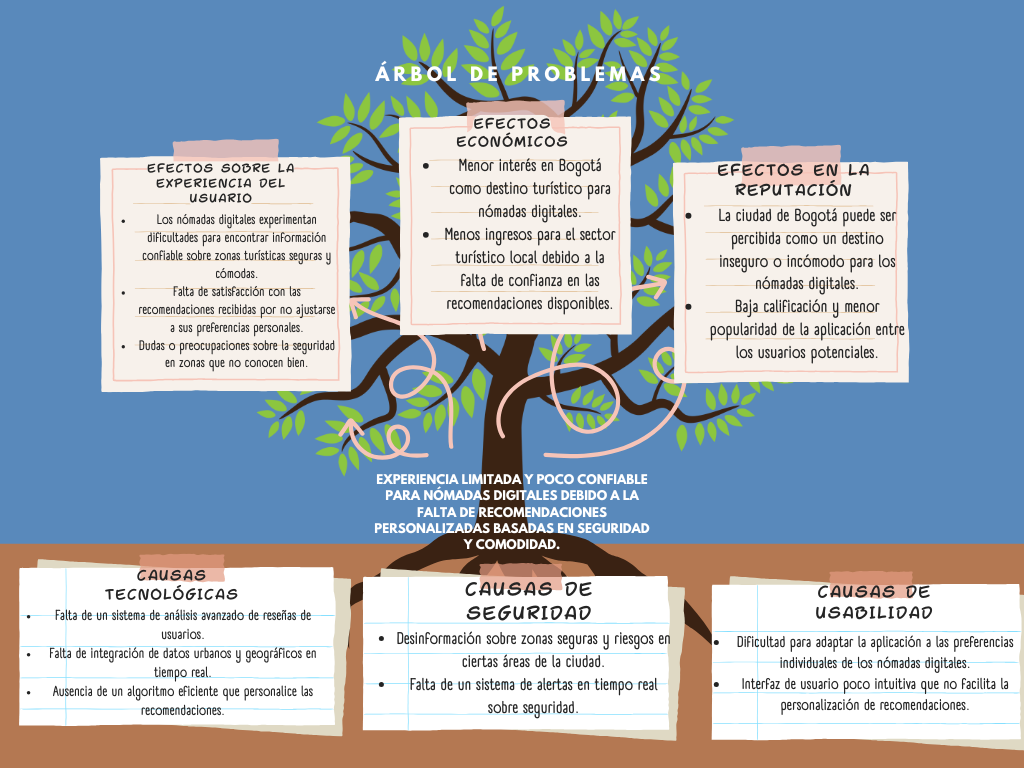
\includegraphics[scale= 0.6]{Content/Images/Gráfica Árbol de problemas Emprendimiento.png}

\end{adjustbox}

\subsection{Descripción del Problema}
Varias compañías del sector de la restauración–Partoo, Superpopi, Healthy Poke, Talent Class y Localboss– se han posicionado públicamente en contra del filtrado de reseñas. Lo consideran como una manipulación que ofrece una visión distorsionada de la realidad a los consumidores. El año pasado, Google eliminó 170 millones de reseñas y 12 millones de perfiles de empresa que no cumplían con su política de contenido, lo que supone un 43\% más que en 2022, según ha contado recientemente la compañía en su blog.\cite{hotelesReseñasNeg}

Esta declaración deja al descubierto como muchas empresas a sabiendas de que es mas fácil modificar deshonestamente sus reseñas haciéndose pasar por clientes conocedores en el tema del turismo que arreglar sus establecimientos y mejorar sus servicios para que cumplan con las expectativas que le plantean en su publicidad.  

Por el otro lado, otra problemática que también se planea mitigar a nivel local con esta oportunidad de desarrollo es la desmeritar reseñas y opiniones que estén fuera de lugar o estén sesgadas negativamente, entiéndase como una “reseña sesgada negativamente” aquella que no abarca una calificación correspondiente a los productos, servicios o experiencia general del cliente ofrecido directamente por una compañía, por ejemplo, no es justo para el emprendedor local que su negocio sea negativamente calificado porque la tienda de al lado hace ruido o el día que estaba consumando su estadía hubo lluvias y no fue de su agrado, este tipo de reseñas perjudica de sobremanera a un establecimiento y esto se evidencia en trabajos de investigación como el realizado por la revista digital Partoo donde se entrevistó a consumidores sobre su frecuencia a revisar reseñas y se llega a la conclusión de que “El 75\% de los encuestados admite que nunca elige un establecimiento con una valoración inferior a 3.5/5” 

\subsection{Formulación del Problema}
¿Cómo aumentar la confianza de los consumidores de aplicaciones digitales de turismo que ha sido afectada por reseñas sesgadas o calificaciones de reseñas manipuladas? 

\subsection{Justificacion del problema}
Después de la rápida caída del sector del turístico a nivel mundial por causa de la pandemia del 2020, Colombia ha tenido una mejora prometedora a partir del 2022 que inclusive ha impulsado notoriamente el desarrollo de este sector aún más que antes de la pandemia. Esta afirmación está respaldada por los datos estadísticos que la Cámara de Comercio de Bogotá puede ofrecer sobre el sector turístico y su desempeño desde principios de 2019 hasta julio de 2024. Para entender el siguiente gráfico es necesario comprender que el éxito del sector del turismo se mide respecto al porcentaje de cupos que ofrecen para sus actividades y estadías. 

\begin{adjustbox}{
    center,
    caption=[{Porcentaje de ocupación mensual: Total nacional y Bogotá}]{\centering Ocupación mensual Bogotá. Fuente: (DANE, Encuesta mensual de alojamiento EMA (enero 2019 - abril 2024))},
    label={ocupaciónmensualbogota},
    nofloat=figure}

    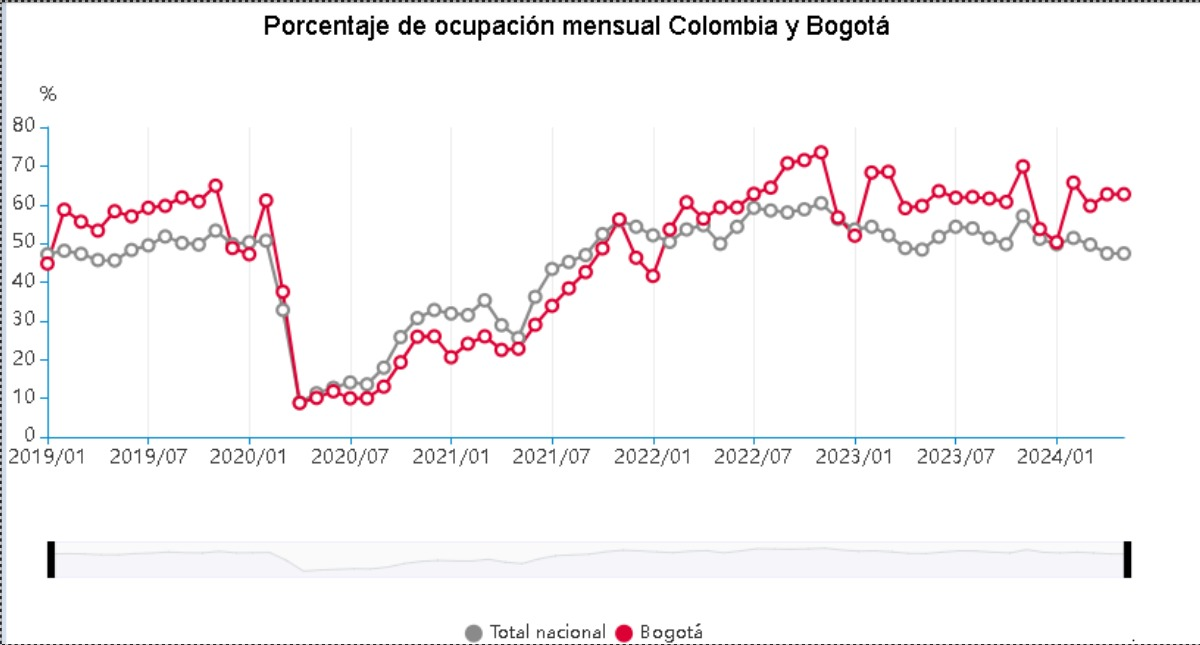
\includegraphics[width=0.2\textwidth]{Content/Images/graficaTurismoBogota.jpeg}

\end{adjustbox}

